\documentclass[11pt]{article}
\setlength{\textheight}{210mm}
\addtolength{\topmargin}{-15mm}
\setlength{\textwidth}{155mm}
\setlength{\oddsidemargin}{5mm}
\usepackage{graphicx, subcaption, amsfonts}
\graphicspath{ {./figs/} }
\pagestyle{plain}
\begin{document}
\title{Dynamics of networks: generation, dimensionality reduction, and coarse-grained evolution of graphs}
\author{\LARGE Proposed by Alexander Holiday\vspace{3mm}\\\Large under the supervision of\vspace{3mm}\\\LARGE Professor Yannis Kevrekidis}
\date{11/01/2013}
\maketitle

\begin{figure}[h]
  \centering
  
\includegraphics[width=0.5\textwidth]{princeton_shield}
\end{figure}

\clearpage
\tableofcontents
\clearpage
\section{Introduction}

\indent From collaborations among movie stars \cite{Barabasi1999} to gene interactions in \texit{C. elegans} \cite{Dreze2009}, network science has found a vast array of applications in the past two decades. This is largely a result of the generality of the network framework: myriad systems are readily adapted to the network description; interacting bodies (e.g. a city, person, or protein) form nodes, the connections between them (e.g. via highways, Facebook friendships, or biological suppresion) create edges. Thus, one may usefully apply the same abstraction to study such disparate topics as the spread of opinions in a society and the kinetics of chemical reactions. \vspace{1mm}\\
\indent However, too often this merely leads to a recasting of the original problem. While this, in itself, can be useful, it fails to exploit the true power in such a formulation. There are several obstacles that prevent the realization of the full utility of networks, a selection of which will be the focus of this proposal. Broadly speaking, the generality of the construct is in some sense its undoing: while numerous problems are addressable, they require many different types of analysis. Thus, a researcher in neural networks may use none of the same tools as a civil engineer designing tranporation networks. Certainly, the dynamics between proteins in a cell and drivers in rush-hour traffic may share almost no similarities; however, this should not prevent investigators in these fields from having similar analytical tools at their disposal.\vspace{1mm}\\ %missing something on dynamics ``of'' and not ``on'', why study ``of''?
\indent One of these methods may be considered a foundation upon which all others rest: the ability to computationally construct networks with desired properties. As the intimate link between a network's underlying structure and its resulting dynamics becomes increasingly evident \cite{Barabasi1999} \cite{Barzel2013}, it becomes difficult to justify the use of simple models in lieu of the ability to construct more accurate versions. Unfortunately, there is currently a lack of methods available to researchers for the construction of networks with desired properties. The algorithms that do exist tend to address a single variable of the network's architecture, leaving others unspecified. Therefore, work remains in creating more general algorithms capable of generating networks with a wide range of structures.\vspace{1mm}\\
\indent Even if one succeeds in accurately modeling a network's structure, the resulting flood of data can be overwhelming and unwieldily to analyze. To address this problem, a class of techniques have been formulated to extract various properties specifically from network systems. These range from community detection algorithms that suggest groupings of similar nodes, to methods that determine the ease with which a signal is propagated in a network \cite{Kleinberg1999} \cite{Newman2004} \cite{Latora2001}. While these have been effective tools in understanding network structure, their applicability is confined to the analysis of single networks. An avenue that has received relatively little attention, and one especially relevant to the study of dynamic systems, is formulating techniques that operate \textit{across} networks. Extending existing methods to operate on \textit{sets} of graphs has the potential to automate the discovery of important parameters governing the evolution of dynamic network systems, revealing their coarse descriptions. This would be a tremendous step forward in network analytics.\vspace{1mm}\\
%% Extracting information from a set of networks presents special challenges, but as the number of temporally-resolvable systems increases, so, too, does the importance of such an ability. Traditional data-mining algorithms such as principal component analysis (PCA), diffusion maps (DMAPS) and nonlinear embedding, can be considered a generalization of the network-analysis tools described above, reducing massive datasets to their significant low-dimensional representations. While more broadly applicable, they currently require that input data be in vector form.
\begin{figure}[h!]
  \centering
  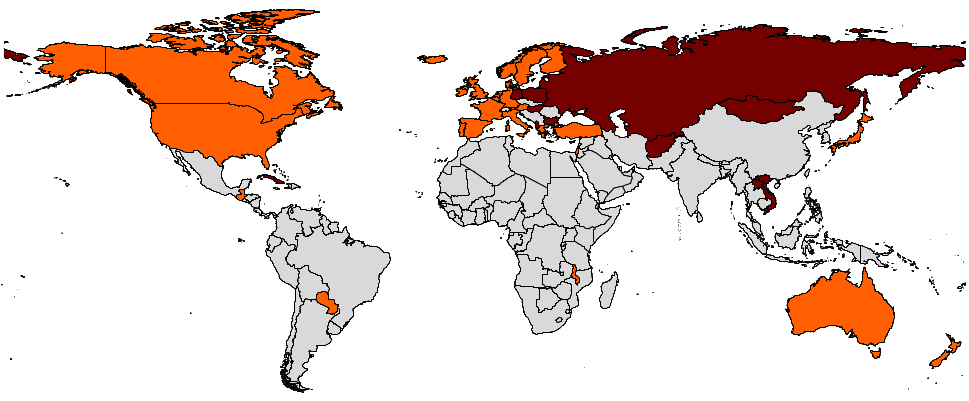
\includegraphics[width=10cm]{unCommunityDetection}
  \caption{Grouping of countries based on United Nations voting records using a community detection algorithm \cite{porter}.}
  \label{fig:un}
\end{figure}
\vspace{1mm}\\
\indent Developing methods that either create specific networks on demand, or determine important system characteristics is, itself, a valuable aim; however, by combining advances in both abilities, we hope to enable various methods of coarse system analysis through \textit{equation free} (EF) \textit{modeling}. The EF framework contains a suite of analytical techniques, from coarse projective integration to systems-level optimization and design. In a field where networks may be composed of billions of nodes, the ability to examine behavior through a low-dimensional system is crucial in reducing simulation times, and allows a fuller analysis of dynamics such as determining fixed point stability and tracking bifurcations.\vspace{1mm}\\
%% EF modeling depends on a key component called the coarse time-stepper, detailed below. In brief, the coarse time-stepper requires a method to a.) discover appropriate macroscopic variables describing system evolution and b.) translate these coarse values into to a fine scale, full simulation. With the data-mining and graph generation techniques to be discussed, we hope to have methods accomplishing both. After implementing the coarse time-stepper, 
\indent Graph generation, detection of signficant features across networks, and EF modeling of complex systems are all interesting avenues of research in their own right. It is hoped that the synthesis of these three elements will allow researchers in a broad range of fields to more accurately model real-world networks, and to attain useful information from subsequent results. We outline each of the three in sections \ref{sec:netGen}, \ref{sec:DM} and \ref{sec:EF}. Section \ref{sec:CW} describes current advances in these topics, while section \ref{sec:FW} concludes the proposal with a discussion of future research plans. Before continuing in this material, the notation used throughout the proposal will be specified.
\section{Notation}
\label{sec:notation}
\indent A graph, $G$, is defined by a set of vertices (or nodes), $V(G)$, and the connections (or edges) between them, $E(G)$. The size of the network, $n \ ( = |V(G)|)$, is the total number of nodes, while the total number of edges is represented by $m \ (= |E(G)|)$. A single vertex, $v_{i}$, is connected to another vertex, $v_{j}$ if and only if the corresponding edge, $e_{ij}$ is non-zero. An edge that begins and ends at the same vertex, $e_{ii}$, is called a loop. If $e_{ij} = e_{ji} \ \forall \ i,j$ then the graph is undirected, i.e. if $i$ is connected to $j$, $j$ must be connected to $i$, e.g. Facebook friendships. Otherwise it is directed. In many cases, the edges take binary values, $e_{ij} \in {0,1}$, and we call the graph unweighted. Alternatively we deal with weighted graphs in which the edge value may take any positive value, typically signifying the strength of connection between $v_{i}$ and $v_{j}$. A reaction network in which edges represent differential equations governing interactions between molecules would be a weighted, directed graph as the interactions between particles could be different, and particle A's influence on B would not imply a reciprocal influence by B on A. This is illustrated in \ref{fig:rxn}. \vspace{1mm}
\begin{figure}[h!]
  \centering
  \begin{subfigure}{.5\textwidth}
    \centering
    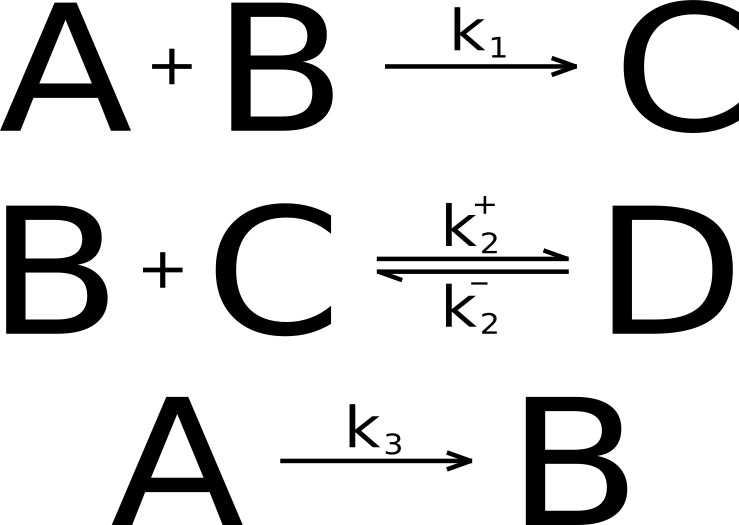
\includegraphics[width=.4\linewidth]{rxnSchematic}
    \caption{}
    \label{fig:rxnSchematic}
  \end{subfigure}%
  \begin{subfigure}{.5\textwidth}
    \centering
    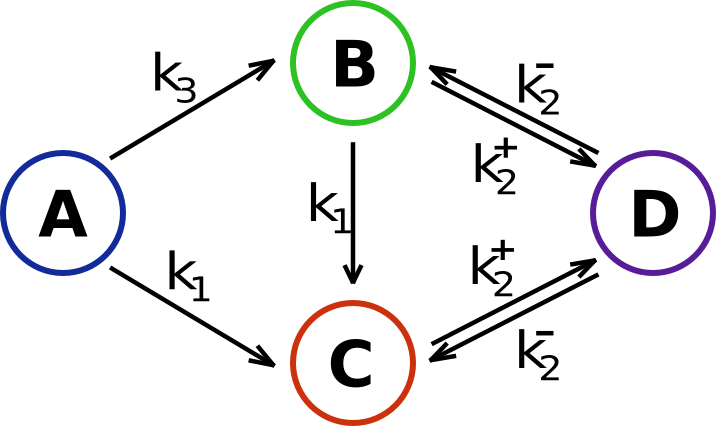
\includegraphics[width=.8\linewidth]{rxnNetwork}
    \caption{}
    \label{fig:rxnNetwork}
  \end{subfigure}%
  \caption{Traditional chemical reaction equation (\ref{fig:rxnSchematic}) and its equivalent reaction network (\ref{fig:rxnNetwork}).}
  \label{fig:rxn}
\end{figure}
\\
There are many ways of specifying a graph, the simplest being a list of all $v_{i}$ and $e_{ij}$ present. However, the most popular method of description is through an ``adjacency matrix'', a square, $n \ \times \ n$, matrix in which $A_{ij}=e_{ij}$. This form is especially helpful when the underlying graph is undirected ($e_{ij}=e_{ji}$) as the adjacency matrix is symmetric. An important property of vertices is their degree, given by $d_{i}=\sum\limits_{j=0}^n e_{ij}$. This measures a node's connectedness in the graph. From the definition, we see that in an unweighted, undirected graph, the degree of a vertex is simply the number of edges connected to it (with loops counted twice). Finally, as no strict definition of a network exists, we use the terms ``graph'' and ``network'' interchangeably. With this foundation, we continue with the original material.
\section{Network Generation}
\label{sec:netGen}
\indent Significant effort has been spent researching algorithms that create networks with different properties. By far the most popular method creates what is called an Erd\H{o}s-R\'{e}nyi random graph. Proposed in 1959 \cite{Erdos1959}, it consists of the following simple procedure: given a set of vertices $V(G)$ and a probability of connection $p$, examine each possible edge in the graph (note there are ${n \choose 2}$ possible edges in an undirected graph) and, with probability $p$, let $e_{ij}=e_{ji}=1$, otherwise $e_{ij}=e_{ij}=0$. Simply put, each edge exists with probability $p$. This straightforward method facilitates theoretical calculations, but, as one might guess, few real-world systems follow such a simplistic scheme. \vspace{1mm}\\
\indent Many different methods of graph generation have been proposed to more accurately capture network structure. They largely fall into two categories: those which describe an evolution of the graph to its final state, and those which generate graphs with specified properties. A famous example of the former is the scale-free preferential attachment model \cite{Barabasi1999}. The method is as follows: begin with a small number of disconnected vertices, $n_{0}$. Add a new vertex, and connect it to $m\le n_{0}$ of the pre-existing vertices. Let the probability that the new vertex, $v_{new}$, connects to one of the old vertices, $v_{old}$, be $P(e_{v_{new}v_{old}}=1)=\frac{d_{old}}{\sum\limits_{i} d_{i}}$. Note that no graph properties have been specified $a\ priori$, except, trivially, the size $n$. In contrast, consider the Erd\H{o}s-R\'{e}nyi model just described. Here, the average degree, $\bar{d}$, is pre-specified, and a graph is constructed that adheres to this stipulation (note that the average degree and the probability of attachment, $p$, are related by $p=\frac{n\bar{d}}{2 {n \choose 2}}$). While the method of evolving a graph to its final form is useful when the underlying growth mechanism is understood, these models are specialized to the system under investigation. When information on the evolutionary process isn't available, as if often the case, it is more useful to measure certain features of the network in question and then use the property-specification class of methods to generate a graph with similar characteristics.\vspace{1mm}\\
\indent The number of such methods, and the variety of properties addressed by them, has grown steadily in recent years. From efficient procedures that generate Erd\H{o}s-R\'{e}nyi random graphs, to those that enable the simultaneous assignment of degree distribution and clustering coefficients \cite{Batagelj2005} \cite{Deijfen2009}, a wide range of variables are tunable in the current collection of methods. The shortcoming of nearly all of the approaches in this toolset is that each addresses only a small number of specific properties. If the network under consideration has a certain degree distribution and contains a specific number of triangles, one must hope that an algorithm has been developed to deal exactly with the creation of a graph with a given degree distribution and triangle count. A method tailored to degree distributions cannot simply be combined with one that specifies the triangle count to achieve the desired outcome. \vspace{1mm}\\
\indent An innovative approach to this problem, the product of collaboration between the Floudas and Kevrekidis groups, aims to alleviate this drawback. Their technique, detailed in \cite{Gounaris2013}, is to formulate the problem as a task for mixed-integer linear optimization. Using this framework, they are able to add property specifications to the algorithm as desired. Each variable that needs to be addressed can be added as a building block in the overall formulation, making the approach tunable to the unique needs of each graph. Additionally, this method can guarantee the non-existence of certain graphs, a useful feature when detailing multiple complex properties. The downside of this wonderful generality is computational slowness. Searching the solution space of all possible graphs can become a daunting task at even modest network sizes of $n=15$ if the searched-for graph is highly detailed. Using certain pre-processing steps, the speed has been greatly increased, but work remains if the method is to be applied to larger systems of $n>100$. 
%possibly remove following figure
\begin{figure}[h!]
  \centering
  \begin{subfigure}{.35\textwidth}
    \centering
    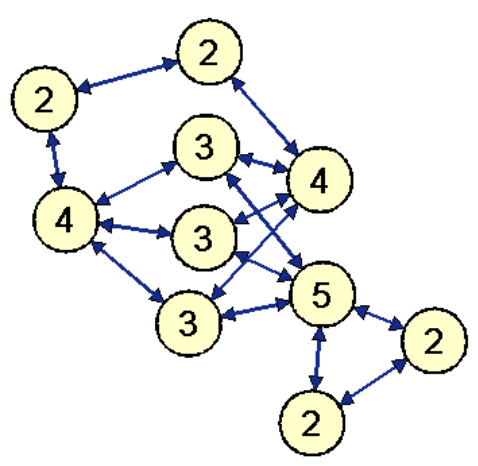
\includegraphics[width=.7\linewidth]{lowCluster}
    \caption{}
    \label{fig:lowCluster}
  \end{subfigure}%
  \begin{subfigure}{.35\textwidth}
    \centering
    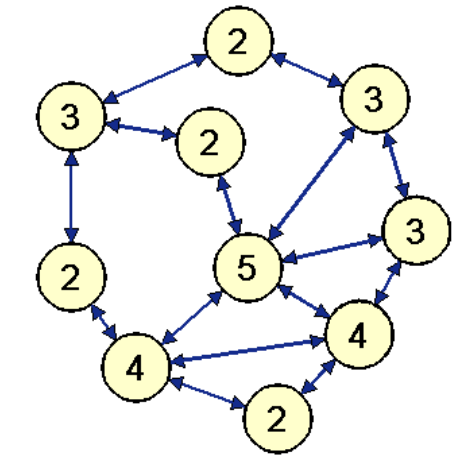
\includegraphics[width=.7\linewidth]{medCluster}
    \caption{}
    \label{fig:medCluster}
  \end{subfigure}%
  \begin{subfigure}{.35\textwidth}
    \centering
    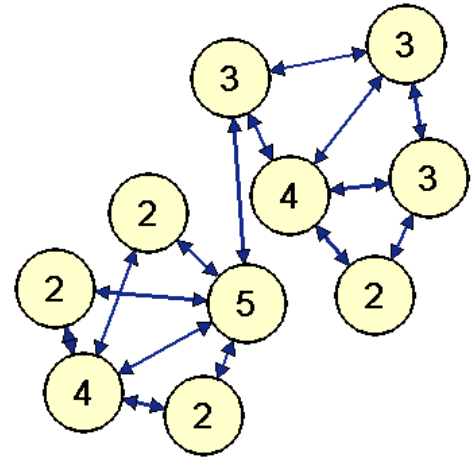
\includegraphics[width=.7\linewidth]{highCluster}
    \caption{}
    \label{fig:highCluster}
  \end{subfigure}%
  \caption{Networks generated by the optimization framework, taken from \cite{Gounaris2013}. The distribution of degrees is identical in both, but the clustering of the nodes was increased from \ref{fig:lowCluster} to \ref{fig:highCluster}.}
  \label{fig:optCluster}
\end{figure}

\vspace{1mm}\\
\indent Certainly, each algorithm has its unique strengths and weaknesses. While some can rapidly construct very large graphs of $n>100,000$, they address only a few of the many potentially interesting properties of a network. The one method that allows users to add properties as desired suffers from scalability issues. The efficient creation of networks with different structural features remains an open area of investigation.
\section{Data Mining across Networks}
\label{sec:DM}
\indent In the past decade, several factors have combined to fuel a wave of algorithms designed to analyze massive data sets. The internet has played no small role, as millions of users give information to online websites wittingly or otherwise, through user accounts or cookies. Additionally, the proliferation of electronic sensors in everything from cars to refridgerators has given companies access to a far greater variety and quantity of information. Crucially, too, spatiotemporal resolution of research experiments has become increasingly commonplace. In these scenarios, data-mining techniques are invaluable in extracting useful information from the resulting massive volumes of data. From the original workhorse of PCA, useful in finding data embedded in linear subspaces, to new, nonlinear manifold learning techniques such as DMAPS, today's techniques exhibit a wide range of approaches to dimensionality reduction \cite{data mining papers}. However, these methods are not currently applicable \textit{across} networks. \vspace{1mm}\\ 
\indent Generally speaking, the goal of a data mining algorithm is to take a collection of points in $\mathbb{R}^{n}$, $n\gg1$ and embed them in $\mathbb{R}^{m}$, $m \ll n$, where the $m$ new dimensions capture the important details of the data. In many cases, data is easily amenable to such a description, e.g. a vector \textit{\{age, longitude, latitude\}} for Amazon users. Unfortunately, when each data point is, itself, a network, there is no clear way to initially ``pre-embed'' each point into $\mathbb{R}^{n}$, and thus the host of techniques proven in other applications become useless. The two options are then to develop new techniques that specifically address the unique aspects of network data, or to devise a scheme that adapts established techniques to operate on graphs. We focus on the latter approach. \vspace{1mm}\\
\indent Many existing methods employ some measure of distance between points in their formulation. For example, a popular implementation of DMPAS requires a weight matrix $W_{ij}=e^{-\frac{\|x_{i}-x_{j}\|^{2}}{\epsilon}}$, in which $x_{i}$ and $x_{j}$ are members of the dataset. Attempting to generalize vector or matrix norms might seem a natural place to start in defining distances between two graphs. As a norm, we would expect $\| x - y \| = 0 \Leftrightarrow x = y$; unfortunately, even determining whether two graphs are equivalent is a complete research puzzle unto itself, and is termed ``the graph isomorphism problem''.
\subsection{Graph isomorphism}
\indent To understand the issue at hand, we must first discuss the distinction between labelled and unlabelled graphs. A labelled graph is one in which the vertices have been assigned a unique identification. In the case of a transportation network of highways between cities, the city names could function as labels. Then, if tasked with determining whether roadways changed between certain points in time, simply checking whether each city's connections remained the same would suffice. One the other hand, vertices in an unlabelled graph have no such intrinsic identity. Comparing two networks is no longer as easy as checking whether all connections to and from each node are the same, as there is no way to identify a node from the first graph, $v_{old}$, with its equivalent, $v_{new}$, in the second. To check whether two unlabelled graphs are different, all possible pairings of nodes from the two graphs may need to be considered. This is the \textbf{NP} problem of determining graph isomorphism, i.e. determining whether two graphs can be labeled in such a way as to make their connections equivalent. Formally, two graphs $G$ and $H$ are isomorphic if there exists a bijective function $f:V(G) \rightarrow V(H)$ such that $v_{i} \in V(G)$ and $v_{j} \in V(G)$ are adjacent if and only if $f(v_{i}) \in H(G)$ and $f(v_{j}) \in H(G)$ are also adjacent. \vspace{1mm}
\begin{figure}[h!]
  \centering
  \begin{subfigure}{.5\textwidth}
    \centering
    \includegraphics[width=.65\linewidth]{graphA}
    \caption{}
    \label{fig:graphA}
  \end{subfigure}%
  \begin{subfigure}{.5\textwidth}
    \centering
    \includegraphics[width=.65\linewidth]{graphB}
    \caption{}
    \label{fig:graphB}
  \end{subfigure}%
  \caption{Different depictions of isomorphic graphs.}
  \label{fig:isoGraphs}
\end{figure}
\vspace{1mm}\\
While a general polynomial-time solver is considered impossible by most as it would prove \textbf{P}$ \ = \ $\textbf{NP}, approximation algorithms with guaranteed error bounds do exist. In fact, polynomial-time solutions are also available, but only for restricted classes of graphs.
\subsection{Graph similarity}
\label{subsec:GS}
\indent Given the difficulty in distinguishing whether two graphs are the same, the challenge in defining a computationally tractable distance measure is understandable. A novel approach to this issue would be to build off existing approximation algorithms. The hope would be to extend one of these methods to output some indication of the differences between graphs, and not just a boolean judgement of ismorphism. This modified method would then be used as the requisite distance measure in pre-existing data mining routines. If this innovative procedure fails, alternative methods have been established in the literature. These are detailed below.
\subsubsection{Edit distance}
\indent The basis of this class of methods is the idea that a graph $G$ is similar to a graph $H$ if $G$ requires few changes, or ``edit operations'', to become identical to $H$. Edit operations consist of adding, removing and relabeling vertices, and adding and removing edges. Each action is assigned a cost, and the total cost of obtaining $H$ from $G$ defines their similarity. Unfortunately, determining the changes in $G$ required to obtain $H$ is computationally infeasible, so different approximations have been developed. In all existing methods, the graph is first converted into a string. This allows string edit distances to be used, which have a stronger theoretical foundation than edit distances of general graphs \cite{Gao2009}. \vspace{1mm}\\
\indent The process of seriation itself is varied, though many approaches use the eigenvector corresponding to the second smallest eigenvalue, i.e. the Fiedler vector, of some transformation of the adjacency matrix. A popular approach frames the problem as the minimization of
\[
g(\pi) = \sum \limits_{i=1}^{|V|} \sum \limits_{j=1}^{|V|} A(i,j)(\pi(i) - \pi(j))^2
\]
for some permutation $\pi$ \cite{Atkins1994}. As minimizing the above is $\textbf{NP-hard}$, the discreet formulation is relaxed in application. Once string representations are determined, any method of string comparison may be used, from string kernels to Dijkstra's algorithm based methods \cite{Hancock2006} \cite{Robles-Kelly2004}. 
\subsubsection{Maximal common subgraph}
\indent Here, the distance between $G$ and $H$ is defined as
\[
d(G,H) = 1 - \frac{|mcs(G, H)|}{max(|G|,|H|)}
\]
where $mcs(G,H)$ is the maximal common subgraph between $G$ and $H$, that is, the largest subgraph of $G$ isomorphic to a subgraph of $H$. This straightforward formula doesn't require the subjective cost function of the edit distance, and is provably a metric on the space of graphs \cite{Bunke1998}. Its computation is, however, $\textbf{NP-hard}$. Nonetheless, heuristics have been employed to use the method in matching chemical structures \cite{Raymond2002}.
\subsubsection{Graph kernels}
\indent A kernel $k(x,x')$ must be symmetric and positive semi-definite; thus, kernels are a less restrictive class of operations compared to metrics, allowing greater freedom formulation. Relatively few graph kernels have been created. Those that have employ random walks over the vertices and edges in their formulation. They have recently been shown to take the general form:
\[
k(G,H) = \sum\limits_{k=0}^{\infty}\mu(k)q_{\times}^{T}W_{\times}^{k}p_{\times}
\]
where $q$ and $p$ are the initial distribution of random walkers and the stopping probabilities, respectively, $k$ is the number of edges traversed during the walk, $W$ represents a sort of combination of $G$ and $H$ known as a product graph, and $\mu(k)$ is a weighting to ensure the sum converges. By defining $\mu(k) = \lambda^{k}$ for some $\lambda$, the infinite sum reduces to the problem of inverting $( \textbf{I} - \lambda W_{\times} )$. This can be computed efficiently in a variety of ways, from conjugate gradients to spectral decompositions \cite{Borgwardt2008}. The downside of these methods is that the value of $\lambda$ defining $\mu(k) = \lambda^{k}$ is often taken to be very small. This ensures convergence of the sum, but neglects higher order terms, i.e. longer walks. The resulting comparison of short walks only captures the local network topology. Defining kernels based on other properties may permit a more holistic measure of graph similarity.
\section{Equation Free Modeling}
\label{sec:EF}
\indent Dynamic network models prescribe behavior at the level of individual vertices and edges, enabling researchers to construct systems with an incredible level of detail. However, while we seek to understand the long-term macroscopic dynamics of the networks, explicit, accurate equations governing this system-level evolution are typically unavailable or poorly understood. To circumvent this need for macroscopic equations in system-level analysis, we turn to \textit{equation free} (EF) \textif{modeling}. However, there are two prerequisites to implementing the EF framework: an appropriate macroscopic description of the network, along with some method of translating these macroscopic variables into realizations of a microscopic system. Advances in the previous sections \ref{sec:netGen} and \ref{sec:DM} would fulfill both. 
\subsection{Coarse time-stepper}
\indent The coarse time-stepper is a basic component of EF modeling, providing the evolution of coarse variables over a short time interval. This is accomplished through controlled initialization of short periods of fine-scale simulations. Define the high- and low-dimensional spaces as $F$ and $C$ (fine and coarse). To move between these two levels of system description, we define the restriction operator $\textbf{R}: F \rightarrow C$, e.g. an extended DMAPS method, and the lifting operator $\textbf{L}: C \rightarrow F$, e.g. some graph generation algorithm. It is important to note that the variables of $C$ may not always provide an accurate representation of the system's fine-scale behavior. Whenever a full simulation is initiated, high-dimensional variables may not be immediately slaved to the low. Instead, a period of ``healing'' is required, after which the system evolves on a slow manifold in $C$. We define this healing interval as $h$. The coarse time-stepper then proceeds as follows:
\begin{enumerate}
\item Initialize a fine-scale simulation at the desired point $u(t_{0}) \in F$.
\item Run the fine-scale simulation to $u(t_{0}+h)$. Behavior can now be described with the low-dimensional variables in $C$.
\item Continue fine-scale simulation, using $\textbf{R}$ to record $n$ collections of coarse variables at intervals of $\Delta t$. 
\end{enumerate}
This provides a time-series of macroscopic variables $\{ \textbf{R(}u(t+k\Delta t) \textbf{)} \}_{k=0}^{n}$. With the ability to investigate low-dimensional dynamics at will, more powerful EF analysis becomes available.
\subsection{Coarse projective integration}
\indent Coarse projective integration (CPI) exploits the assumed smoothness of the coarse variables' evolution to accelerate simulations. Define the coarse variable $U \in C$. The procedure is outlined as:
\begin{enumerate}
\item Run the coarse time-stepper to record the coarse timeseries $\{ U_{t} \}_{t=t_{0}}^{t_{f}}$.
\item Using this collection, numerically calculate $\frac{dU}{dt}(t_{f})$.
\item With some integration routine, e.g. Euler' method, project $U$ forward to some $U_{new} = U_{t_{f}+\Delta t}$.
\item Lift $U_{new}$ to $u = \textbf{L}(U_{new})$.
\item Iterate these previous steps until the desired system state is reached.
\end{enumerate}
By projecting forward the few variables that evolve smoothly on the system's slow manifold, expensive, full simulation is significantly reduced. The result is a steep improvement in computation time.
\subsection{Coarse fixed point calculations}
\indent Given a macroscopic state $U_{n} \in C$, let $U_{n+1} = \Phi_{T}(U_{n})$ be the state of the system after time $T$. A fixed point could be evaluated by locating $g^{*}$ such that 
\[
F(U^{*}) = U^{*} - \Phi_{T}(U^{*}) = 0
\]
Typically, as in Newton-Raphson iteration, the derivatives $\frac{dF}{dU}$ would be needed to update the solver. While certainly not available analytically, these derivatives can be approximated numerically. This is an effective but expensive task, as it requires the repeated use of the coarse time-stepper. Using fixed point methods like the generalized minimization of residuals (GMRES) would improve performance \cite{Saad1986}.
\subsection{Coarse bifurcation analysis}
Once a steady state has been found, we may track its dependence on system parameters to analyze system bifurcations. This can be accomplished, for example, by a pseudo-arclength continuation scheme. Define $\lambda$ as the system parameter and $s$ the arc-length along the $\|U\|$ vs. $\lambda$ bifurcation curve, i.e. $s$ parameterizes $U(s)$ and $\lambda(s)$. Then, if we know the solution at some point $s_{0}$, we may solve the following system to find the values of $U(s_{0}+ds)$ and $\lambda(s_{0}+ds)$:
\[
F(\textbf{U}, \lambda) = 0 \\
\]
\[
\| \frac{d \lambda}{ds}(s_{0}) \|^{2} + \| \frac{d \textbf{U}}{ds}(s_{0}) \|^{2} = 1
\]
\section{Current Work}
\indent Initial research has focused on accelerating simulations of dynamical network systems. While leaping to the third of three steps may seem premature, it quickly reveals weaknesses in the overall process of simulation, and serves as a guide for future investigation. Two cases were studied, a voting model with possible applications in sociology, and an edge reconnecting model, which mainly serves as a toy mathematical network for which behavior can be derived analyticaly. After briefly describing the dynamics of each, current progress in simulation acceleration will be discussed.

\subsection{Voting model}
\indent The \textit{k} opinion voter model initally consists of an Erd\H{o}s-R\'{e}nyi graph of size $n \ >10,000$, with small average degree, $\bar{d}\asymp 1$. To begin, each vertex is randomly assigned an opinion based on some initial distribution $\{p_{i}\}_{i=1}^{k}$. With this initial state and a ``probability of reattachment'' $\alpha$, the graph evolves as follows (note that $\zeta(v_{i})$ denotes the opinion of $v_{i}$):
\begin{enumerate}
\item Choose an edge $e_{ij}$ uniformly at random from $E(G)$.
\item Randomly choose one of the endpoints of $e_{ij}$, call it $v_{i}$. The other endpoint will be $v_{j}$.
\item Repeat steps one and two until $\zeta(v_{i}) = \zeta(v_{j})$, i.e. the vertices' opinions do not match.
\item With probability $\alpha$, remove $e_{ij}$ from the graph.
\begin{enumerate}
\item Choose a new vertex $v_{k}$ uniformly at random from $V(G)$ until $e_{ik} \notin E(G)$.
\item Add $e_{ik}$ to $E(G)$.
\end{enumerate}
\item Otherwise, with probability $1-\alpha$, set $\zeta(v_{i}) = \zeta(v_{j})$.
\end{enumerate}

\begin{figure}[h!]
  \centering
  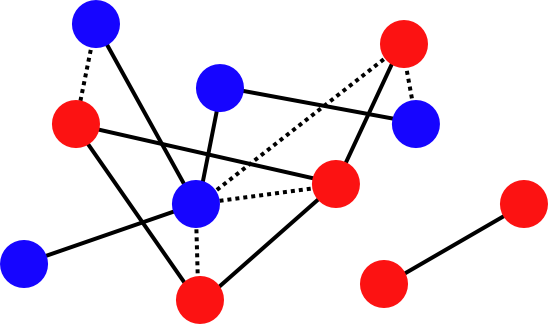
\includegraphics[width=.5\linewidth]{votingModel}
  \caption{A possible configuration of a two-opinion model. The dotted lines represent conflicts. We may take the blue nodes to be Democrats, the red Republicans; then, the highly connected blue node may represent President Obama, the isolated red component Michele Bachmann and Sarah Palin.}
  \label{fig:graphA}
\end{figure}
\\
This process is iterated until the system reaches a consensus state in which $\zeta(v_{i}) = \zeta(v_{j}) \ \forall \ v_{i}, v_{j} \in V(G)$, i.e. every edge connects vertices of the same opinion. An edge $e_{ij}$ is called a conflict whenever $\zeta(v_{i}) \ne \zeta(v_{j})$. Thus the system is evolved until all conflicts are removed. While the general \textit{k} opinion model has received some attention \cite{Shi}, our focus will be the simpler two opinion model. In this case, it has been shown that, for a certain initial minority fraction $p_{minority} \le 0.5$, a bifurcation occurs as $\alpha$ increases. At low values of $\alpha$, fewer edges are rewired and the system approaches a static state. In this limit, the system should converge once each of the $m$ edges are selected, which occurs in $O(n\sqrt{n})$ steps  \cite{Durrett2012}. As $\alpha$ increases, so does The frequency of rewiring edges. This slows the rate of consensus to $O(n^{2})$. Interestingly, besides differences in convergence speed, the final consensus state also changes. In the low-$\alpha$ limit, the final minority fraction is an increasing function of $\alpha$. In the slower, high-$\alpha$ range, the final minority fraction is unchanged from its initial value. Fig. \ref{vmBifDiag5000} illustrates the effect of $\alpha$ and $p_{minority}$ on the final consensus state.\vspace{1mm}
\begin{figure}[h!]
  \centering
  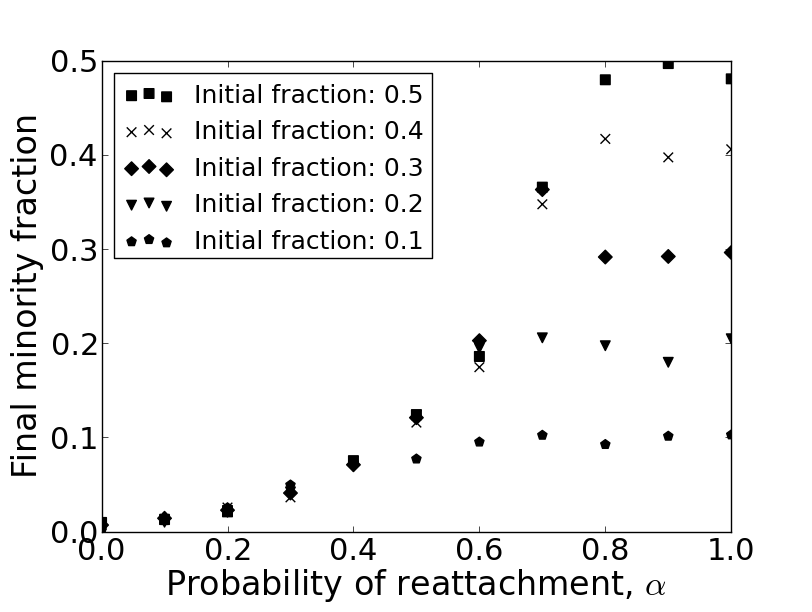
\includegraphics[width=.5\linewidth]{vmBifDiag5000}
  \caption{The effects of $\alpha$ and initial minority fraction on the final state. Above $\alpha \approx 0.8$, the final and initial fractions are approximately equal. Below this, a curve is mapped out. Any initial minority fraction above the curve will evolve towards the steady state value below.}
  \label{fig:vmBifDiag5000}
\end{figure}
\begin{figure}[h!]
  \centering
  \begin{subfigure}{.5\textwidth}
    \centering
    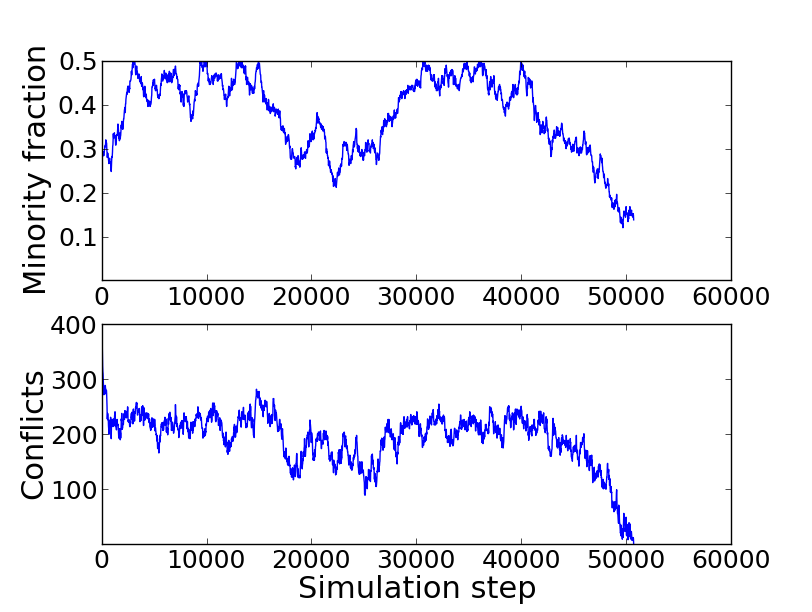
\includegraphics[width=1.0\linewidth]{vmSlaving}
    \caption{}
    \label{fig:vmSlave}
  \end{subfigure}%
  \begin{subfigure}{.5\textwidth}
    \centering
    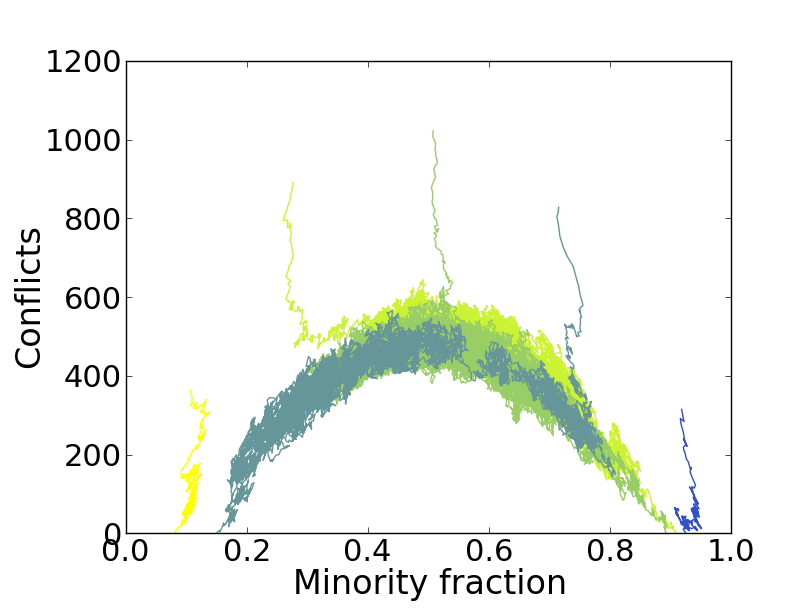
\includegraphics[width=1.0\linewidth]{vmPhasePlotv2}
    \caption{}
    \label{fig:vmPP}
  \end{subfigure}%
  \caption{Evolution of minority fraction and number of conflicts, \ref{fig:vmSlave}, and phase plot, \ref{fig:vmPP}. Note  the strong correlation between the minority fraction and conflict evolution in \ref{fig:vmSlave}.}
  \label{fig:vmResults}
\end{figure}
\\
\indent By creating phase plots of different system properties, it was observed that the minority fraction dictates the state of the system. Fig. \ref{vmSlave} illustrates that the number of conflicts could be written as a function of the minority fraction, while \ref{vmPP} shows the independence of initial and final minority fractions. This suggested that the system minority fraction could serve as a macroscopic variable in CPI. The system is stochastic; thus,  in order to obtain smooth evolutions of variables, the average trajectory of an ensemble of voting models was used. In fact, both the minority fraction and conflict count were used as coarse variables. After projecting these variables forward in macroscopic space, it remained to generate a graph with a specific minority fraction and conflict count. Thankfully this was a simple task, and a customized algorithm was developed. CPI results are shown in Fig. \ref{vmResults}.\\
\begin{figure}[h!]
  \centering
  \begin{subfigure}{.5\textwidth}
    \centering
    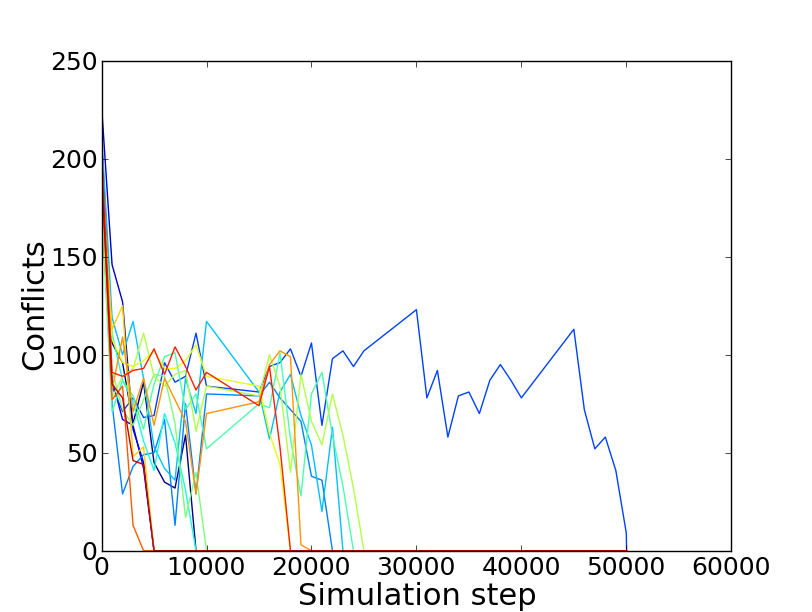
\includegraphics[width=1.0\linewidth]{vmCPI16v2}
    \caption{CPI in an ensemble of 16 simulations}
    \label{fig:vmCPI}
  \end{subfigure}%
  \begin{subfigure}{.5\textwidth}
    \centering
    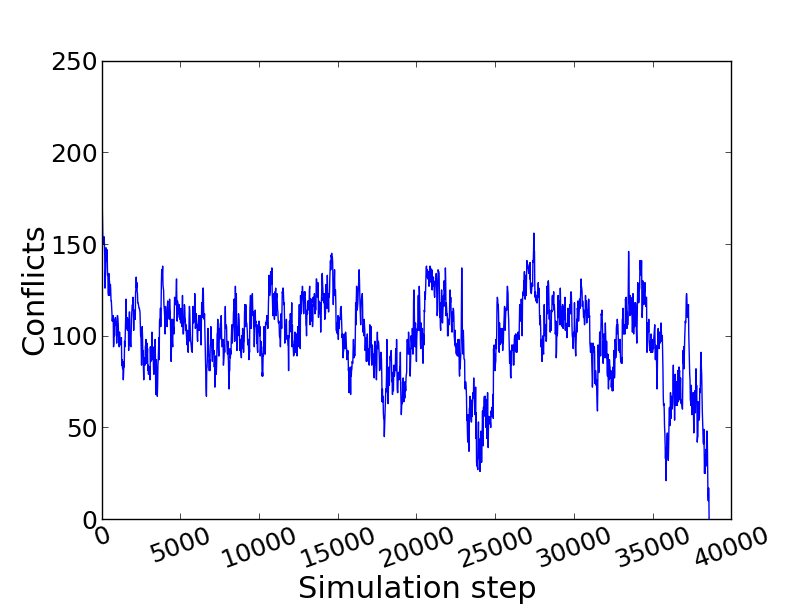
\includegraphics[width=1.0\linewidth]{vmSingleLongTC}
    \caption{Direct simulation}
    \label{fig:vmNoCPI}
  \end{subfigure}%
  \caption{System evolution with and without CPI. Note that initially in \ref{fig:vmCPI}, with many trajectories averaged together, a large number of models quickly converge. However, the remaining runs become somewhat erratic as they lose the dampening effect that averaging with many simulations had provided. In both cases, $n=200$.}
  \label{fig:vmResults}
\end{figure}
\subsection{Edge reconnecting model}
\indent The edge reconnecting model, proposed in \cite{Rath2012}, presents special difficulties in creating accurate low dimensional representations of the overall system. Namely, the network is allowed to have multiple edges connecting the same vertices. Such a construction is termed a ``multigraph''. Initially, $m\asymp n^{2}$ edges are distributed uniformly among the $n$ vertices. Then the multigraph evolves as a Markov chain according to the following dynamics:
\begin{enumerate}
\item Choose an edge $e_{ij} \in E(G)$ uniformly at random and flip a coin to label one of the ends as $v_{i}$
\item Choose a vertex $v_{k}$ using linear preferential attachment: $P(v_{k} = v_{l}) = \frac{d_{l}}{\sum\limits_{i=1}^{n} d_{i}}$
\item Replace $e_{ij}$ with $e_{ik}$
\end{enumerate}
This process is repeated until a frozen state is reached, at which point the degree distribution remains constant.\vspace{1mm}\\
\indent Interestingly, while the network is strictly unlabeled, the preferential attachment dynamics tend to stratify the vertices into a low degree majority and extremely high degree minority. This permits a sort of pseudo labeling of the vertices, as a vertex of high (low) degree at time $t_{1}$ is likely to retain its high (low) degree at $t_{2}$. Therefore, when sorted by degree, the evolution of the adjacency matrix appears smooth, as shown in Fig. \ref{fig:paAdjSort}. \vspace{1mm}\\
\indent Two distinct timescales arise from these dynamics, $T\asymp n^{2}$ and $T\asymp n^{3}$ where $T$ is the number of steps. On the faster, $O(n^{2})$ scale, the degrees of the vertices may be considered constant, while the number of parallel edges between vertices changes. On the slower $O(n^{3})$ scale, the degree distribution evolves to a steady state value. While these separate timescales have been proven in \cite{Rath2012}, identifying them through numerical simulations is complicated by a couple of factors. First, the exact timescales themselves are difficult to discern. Both scales are really $O(\rho_{1} n^{2})$ and $O(\rho_{2} n^{3})$, where the constants $\rho_{i}$ are evaluated at the limit of infinite-sized graphs, $n\rightarrow \infty$. This hints at the second, larger, problem: many of the results on the existence of these timescales in the first place are only valid in this large-$n$ limit. Simulation time then becomes problematic. Figs. \ref{fig:paN2} and \ref{fig:paN3} illustrate attempts to visualize these separate scales of evolution. The changes in each appear quite gradual, and no distinct timescales are evident.\\
\begin{figure}[h!]
  \centering
  \begin{subfigure}{.5\textwidth}
    \centering
    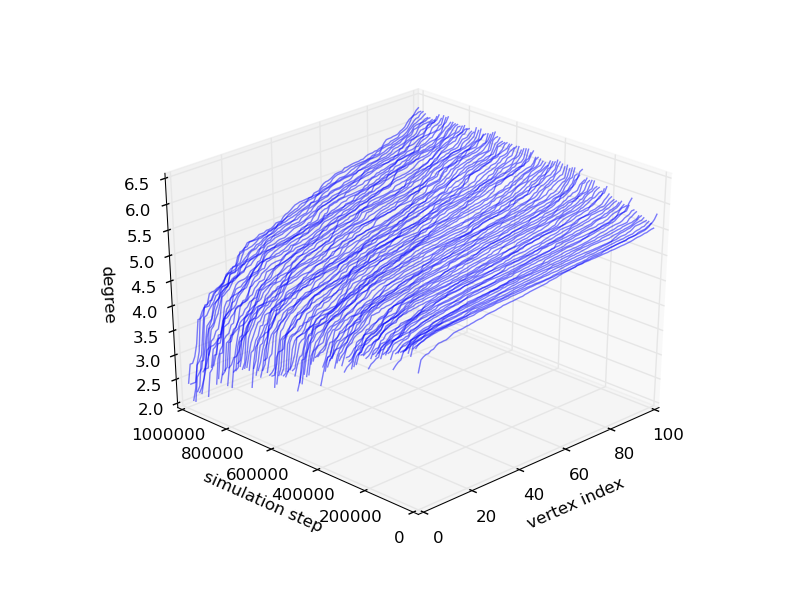
\includegraphics[width=1.0\linewidth]{nSquaredTimescale}
    \caption{}
    \label{fig:paN2}
  \end{subfigure}%
  \begin{subfigure}{.5\textwidth}
    \centering
    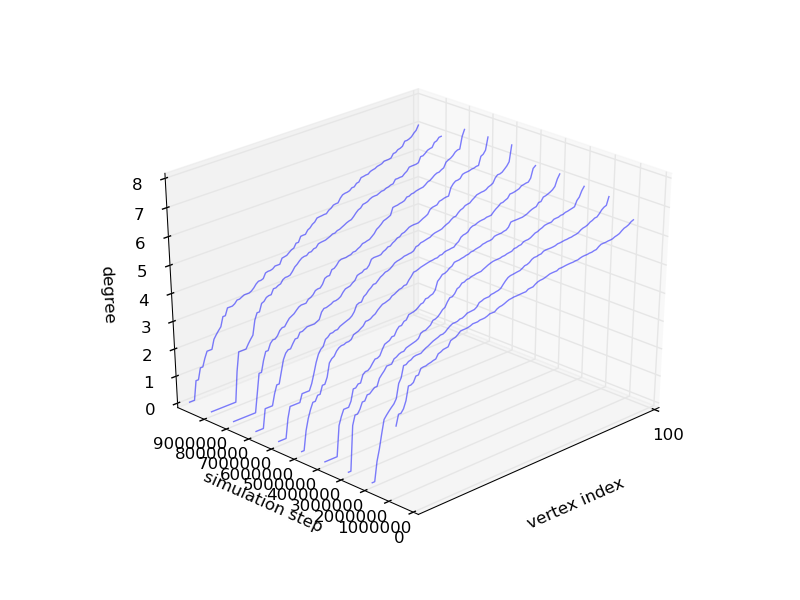
\includegraphics[width=1.0\linewidth]{nCubedTimescale}
    \caption{}
    \label{fig:paN3}
  \end{subfigure}%
  \caption{Degree evolution on $n^{2}$ and $n^{3}$ timescales, in \ref{fig:paN2} and \ref{fig:paN3} respectively.}
  \label{fig:vmResults}
\end{figure}
\indent Our approach in coarse-graining system dynamics is based on the existence of a gap in the spectrum of the adjacency matrix, and the subsequent ability to approximate $A\approx \lambda_{1}v^{(1)}v^{(1) \;\dagger}$ where $A$ is the adjacency matrix of the system, $\lambda_{1}$ is the leading eigenvalue of $A$, and $v^{(1)}$ the corresponding eigenvector.
\begin{figure}[h!]
  \centering
  \begin{subfigure}{.5\textwidth}
    \centering
    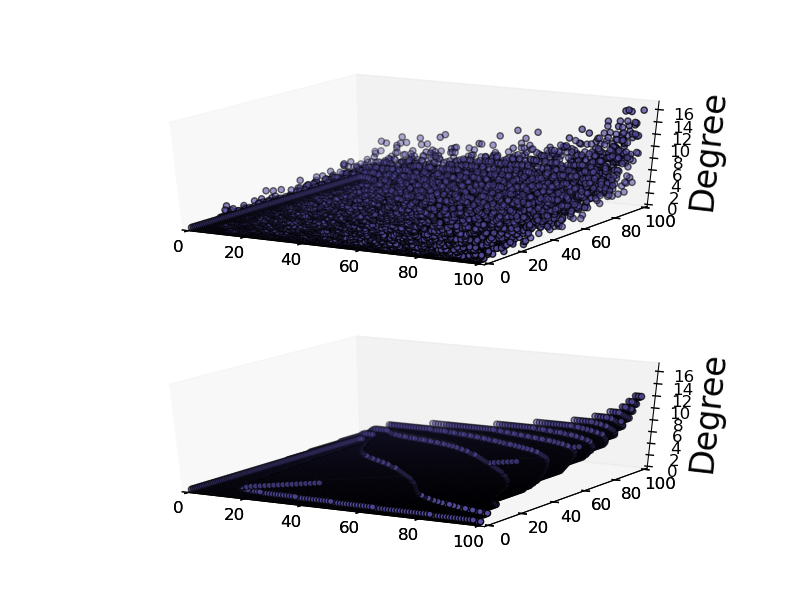
\includegraphics[width=0.7\linewidth]{paRecon}
    \captionsetup{width=0.8\textwidth}
    \caption{Reconstruction of original adjacency matrix (top) using first eigenvalue/eigenvector pair (bottom).}
    \label{fig:paRecon}
  \end{subfigure}%
  \begin{subfigure}{.5\textwidth}
    \centering
    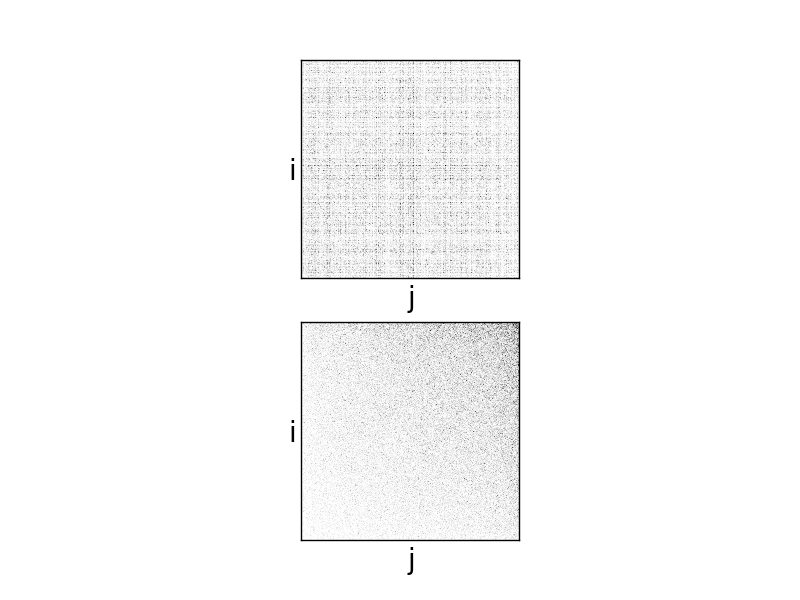
\includegraphics[width=0.7\linewidth]{paAdjSort}
    \captionsetup{width=0.8\textwidth}
    \caption{The unsorted adjacency matrix appears random (top), but sorting by vertex degree reveals its structure (bottom).}
    \label{fig:paAdjSort}
  \end{subfigure}%
  \caption{Reconstruction of adjacency matrix, \ref{fig:paRecon}, and vertex sorting, \ref{fig:paAdjSort}.}
  \label{fig:paAdj}
\end{figure}
\\
Fig. \ref{fig:paRecon} illustrates the reconstruction of the adjacency matrix as $A_{ij}=\lambda_{1}v^{(1)}_{i}v^{(1) \;\dagger}_{j}$ (after multiplication, each entry $A_{ij}$ was rounded to the nearest integer if $i\neq j$ or to the nearest even integer if $i=j$). Visually, the two correspond very well. \\
\indent As $\lambda_{1}v^{(1)}v^{(1) \;\dagger}$ appeared a good approximation of $A$, it was reasoned that we could use this eigenvalue/eigenvector combination as a coarse description of the system. In order to further reduce dimensionality, the eigenvector was fitted with a fifth-degree polynomial. Five degrees were used as additional terms didn't significantly increase fitting accuracy. The six coefficients of this function were then used as a smaller set of coarse variables, leading to a final seven-dimensional representation of the system (six coefficients plus an eigenvalue). The following outlines the CPI framework:
\begin{enumerate}
\item Simulate the full edge reconnecting model dynamics for some number of steps until the fast variables are sufficiently slaved to the slow.
\item Record the adjacency matrix as the system evolves on the slow manifold.
\item Project forward the coarse variables (coefficients and eigenvalue).
\item Reconstruct a new adjacency matrix from the new, projected coefficients and eigenvalue:
  \begin{enumerate}
  \item Compute a new eigenvector as $v(i) = \displaystyle\sum\limits_{k=0}^{k=6} i^{k}c_{k}$ (where $c_{k}$ represents the coefficients of the polynomial and $v(i)$ the $i^{th}$ component of $v$) and round to the nearest integer
  \item Compute the new adjacency matrix as $A_{ij}=\lambda_{1}v^{(1)}_{i}v^{(1) \;\dagger}_{j}$ and round as discussed previously
  \end{enumerate}
\item Repeat from step one until system reaches steady state
\end{enumerate}
Preliminary results of this method are shown in Fig. \ref{fig:paCPI}, in which the evolution of the degree distribution is shown for both the full simulation and a simulation in which CPI has been employed. The two generally coincide.\\
\begin{figure}[h!]
  \centering
  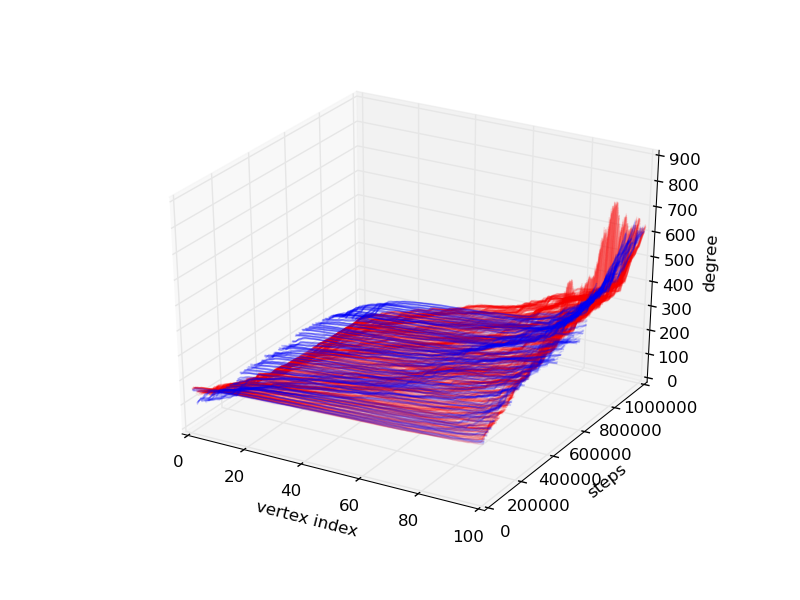
\includegraphics[width=0.6\linewidth]{paCPI}
  \caption{Overlay of direct simulation (red) and CPI (blue).}
  \label{fig:paCPI}
\end{figure}
\section{Future Work}
A number of areas present themselves as good research directions. They're divided by subject below.
\subsection{Graph generation}
\indent We will start by re-examining the recent optimization based method of graph generation. The main limitation of the approach is its scalability. Preprocessors have been shown to significantly reduce runtimes, but have been created to address specific properties \cite{Gounaris2011}. These operate by removing search paths unlikely to yield the specified graph before the optimization algorithm begins. This works particularly well when many distinct (non-isomorphic) graphs exist that satisfy the stipulations. In this case, the preprocessor does not need to be particularly careful in its deletions, as it is unlikely to remove all branches leading to feasible solutions. When more specificity is needed, it is possible to tune this step to be more cautious in its selections. Creating a generic preprocessor for arbitrary properties would retain the generality of the method while increasing speed. \\
\subsection{Data mining across networks}
\indent This nascent research topic has received little attention. Certain sub-problems, e.g. graph isomorphism, graph matching, and vertex matching, have been thoroughly investigated; but, the concept of applying dimensionality techniques when data points are, themselves, networks seems new. As mentioned, it may be possible to adapt an existing approximation algorithm that determines graph isomorphism to additionally yield information on the differences between two networks. A thorough understanding of the structure of these methods through an extensive literature review will be a necessary starting point. \vspace{1mm}\\
\indent Alternatively, the computer science community has established a number of graph similarity methods, as outlined in \ref{subsec:GS}. If these test poorly, the most promising direction wouldappear to be in defining new kernels between graphs. The foundation of these graph kernels is a paper from 1999 \cite{Haussler1999} which provides a general framework from which other kernels could be invented. \vspace{1mm}\\
\indent In general, work would focus on developing graph similarity measures in simple models, such as Erd\H{o}s-R\'{e}nyi, in which issues would be more readily diagnosed and guarantees of success or failure more easily proven. Additionally, simpler, heuristic measures of graph similarity have been shown to work in certain scenarios. These could be used while more grounded methods are developed, or a combination of simple measures could be found that adequately addresses our needs.
\subsection{Equation free modeling}
\indent The immediate aim in this direction will be to apply diffusion maps to the voting model data in an attempt to recover the minority fraction as a good coarse variable. This is expected to work, as DMAPS has been able to discover appropriate coarse variables in other collections of graphs using heuristic similarity measures. It would also be useful to apply the coarse fixed point calculations to the edge reconnecting model, as direct simulations are computationally intensive.

\bibliographystyle{abbrv}
\bibliography{$HOME/Documents/bibTex/library}
\end{document}
